%! Author = WelJo
%! Date = 8/18/2026

\section{Implementation}
\label{sec:implementation}

Evaluating dynamic accessibility across thousands of origins over 336 hourly timesteps is computationally intractable if spatial overlays are computed dynamically at runtime.
Our Python 3.10 pipeline decouples heavy geospatial precomputation from discrete-time simulation for municipal Trier, Germany ($117\,\text{km}^2$), integrating open geospatial data with official hydrodynamic flood models.


\subsection{Hydrodynamic Stage Ingestion and Spatial Preprocessing}
\label{subsec:data-ingestion}

\subsubsection{Multi-Stage Hydrodynamic Ingestion (\texttt{HQ\_raw}):}
Our hazard model digests empirical hydrodynamic flood stages from the Rhineland-Palatinate Water Management Authority.
The dataset (\texttt{HQ\_raw}) comprises $29$ discrete gauge shapefiles (\texttt{Pegel\_09\_00m} to \texttt{Pegel\_11\_80m}), spanning gauge heights from $9.00\,\text{m}$ to $11.80\,\text{m}$ (HQ100 peak) in $0.10\,\text{m}$ increments~\cite{trier_geodaten}.
In \texttt{flood\_interpolation.py}, the ingestion routine projects geometries to WGS84 (\texttt{EPSG:4326}) and UTM Zone 32N (\texttt{EPSG:25832}), dissolving adjacent tiles via \texttt{shapely.ops.unary\_union} into unified stage polygons $\mathcal{P}_k$ ($k \in [0, 28]$) cached under \path{data/processed/flood_interpolation/}.

\subsubsection{Multimodal Infrastructure and Network Ingestion}
Infrastructure within Trier ($\sim 117\,\text{km}^2$) is extracted from OpenStreetMap via \texttt{OSMnx}:
(1)~\textbf{Road Network ($G$)}: Filtered to drivable roads, yielding an undirected graph of $|V| = 5{,}817$ nodes with traversal times $c(e) = \text{length}(e)/\text{speed}(e)$.
(2)~\textbf{Critical POIs and Utilities}: Destinations comprise $3$ acute hospitals and $12$ fire stations.
Coupled utilities encompass $131$ power assets ($\mathcal{I}_{\text{power}}$, substations and plants) and $11$ water assets ($\mathcal{I}_{\text{water}}$, waterworks, towers, pumping stations).
Facility footprints are converted to interior representative points $\mathbf{p}_i$ and snapped to nearest network vertices $\pi(\mathbf{p}_i) \in V$ via R-tree queries.


\subsection{System Architecture and Execution Pipeline}
\label{subsec:system-architecture}

\subsubsection{Modular Architecture and Technology Stack}: The pipeline couples five sequential modules: spatial ingestion, hazard overlay analysis, utility dependency mapping, temporal simulation, and scenario evaluation.
The software foundation combines \texttt{GeoPandas} and \texttt{Shapely} (geometry and spatial indexing), \texttt{OSMnx} and \texttt{NetworkX} (graph extraction and routing), and \texttt{NumPy} (vectorized state matrices).
As shown in Figure~\ref{fig:pipeline}, data flows unidirectionally through persistent disk caches into \texttt{dynamic\_roa.py}.

\begin{figure}[htbp]
    \centering
    \vspace{-2.5mm}
    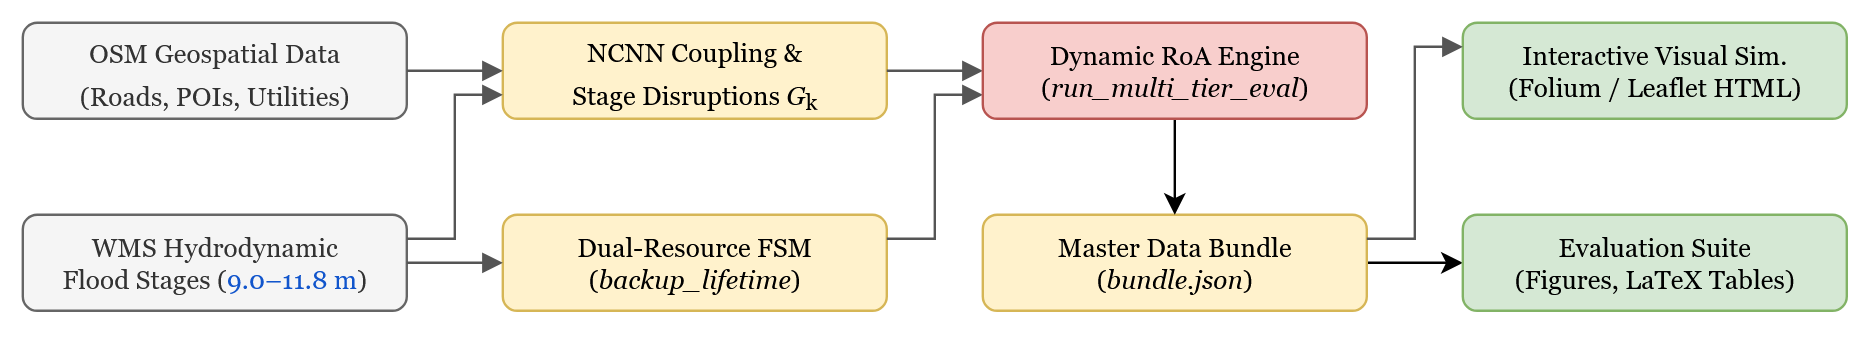
\includegraphics[width=0.96\linewidth]{resources/pipeline}
    \vspace{-2.5mm}
    \caption{Modular architecture: Precomputed stage subgraphs and FSM trajectories feed the dynamic RoA simulation engine, producing a master data bundle.}
    \label{fig:pipeline}
    \vspace{-3.5mm}
\end{figure}

\vspace{-\topsep}

\subsubsection{Two-Phase Pipeline Paradigm:}
Naively intersecting road edges with flood polygons across $1{,}344$ hourly tier evaluations is expensive.
Our architecture enforces a two-phase paradigm:
\textbf{Phase~1 (Spatial Preprocessing)} executes heavy geometric operations, network extraction, boundary aggregation, edge disruption slicing, and utility routing (NCNN), once per study area, caching all cut-sets under \path{data/processed/}.
\textbf{Phase~2 (Dynamic Simulation)} loads cached lookups into memory, evaluating FSM transitions and accessibility over 336 hours in seconds without geometric operations.

\subsection{Direct Flood Determination and Network Disruption Mapping}
\label{subsec:hazard-mapping}

\subsubsection{Facility Inundation via Interior Representative Points}
Determining facility inundation requires robust geometric testing.
Standard centroids and bounding envelopes fail on complex non-convex footprints (e.g., L-shaped hospitals): centroids drift into dry courtyards, while bounding boxes trigger false positives when floodwaters overlap parking lots.
In \texttt{flood\_status.py}, the representative\_point() method guarantees test coordinates lie strictly within the interior: $\mathbf{p}_i \in \text{Int}(\text{Geom}_i)$.
Vulnerability across all 29 stages is evaluated via GeoPandas spatial R-trees (\texttt{sindex}) in $\mathcal{O}(\log |\mathcal{D}|)$ time and cached as direct flood matrices.

\subsubsection{Road Network Edge Disruption and Cut-Sets}
Dynamic accessibility degradation depends on road passability.
In \texttt{stage\_disruptions.py}, graph edges are intersected against each stage polygon $\mathcal{P}_k$.
To preserve elevated river crossings, edges with a non-null \texttt{bridge} tag remain open unless flood heights submerge bridge decks.
Flooded edge tuples $(u, v, \text{key})$ form stage cut-sets $E_{\text{flood}, k} \subset E$, cached in JSON format.
Passable subgraphs $G_k = (V, E \setminus E_{\text{flood}, k})$ are instantiated in memory in $\mathcal{O}(|E_{\text{flood}, k}|)$ time, bypassing geometric clipping entirely.

\subsubsection{Network-Constrained Utility Routing (NCNN)}
Because utility conduits follow street corridors underground, Euclidean distance distorts real infrastructure dependencies across river barriers.
In \texttt{ncnn.py}, dependency assignment $s^*(i, r)$ for facility $i \in \mathcal{D}$ and resource $r \in \{\text{power}, \text{water}\}$ is computed on base graph $G_0$ in UTM Zone 32N (\texttt{EPSG:25832}).
To avoid pairwise queries, a multi-source Dijkstra traversal (\texttt{nx.multi\_source\_dijkstra}) runs from all utility assets $\mathcal{I}_r$ simultaneously, mapping each facility node $\pi(\mathbf{p}_i)$ to its nearest utility in $\mathcal{O}(|E| + |V|\log |V|)$ time.
Reconstructed paths are cached under \path{data/processed/ncnn/}, coupling facility FSM states to upstream utility flooding.

\subsection{Two-Tier Caching Strategy and Storage Hierarchy}
\label{subsec:caching-strategy}

\subsubsection{On-Disk Directory Hierarchy and Naming Conventions}
Intermediate spatial artifacts are persisted under \path{data/processed/} (Table~\ref{tab:cache_hierarchy}) using deterministic keys \texttt{<type>\_<place>\_<K>\_<T>h.<ext>} ($K=29, T=336\,\text{h}$), preventing stale cache reads across experiment setups.

\begin{table}[htbp]
    \centering
    \vspace{-2.5mm}
    \caption{Persistent on-disk cache hierarchy under \texttt{data/processed/}.}
    \label{tab:cache_hierarchy}
    \scriptsize
    \renewcommand{\arraystretch}{0.95}
    \begin{tabularx}{\textwidth}{l l X}
        \hline
        \textbf{Pipeline Phase} & \textbf{Subdirectories} & \textbf{Key Artifacts and Stored Data} \\
        \hline
        Hazard Preprocessing & \path{flood_interpolation/}, \path{network/} & 29 dissolved flood polygons $\mathcal{P}_k$; road cut-sets $E_{\text{flood}, k}$. \\
        Spatial Coupling & \path{services/}, \path{flood_status/}, \path{ncnn/} & Snapped POIs; stage inundation matrices; NCNN paths. \\
        Temporal Simulation & \path{backup_lifetime/}, \path{roa/} & Hourly FSM buffer logs; multi-tier evaluation bundle. \\
        \hline
    \end{tabularx}
    \vspace{-3.5mm}
\end{table}

\vspace{-\topsep}

\subsubsection{Computational Complexity Reduction}
Un-cached accessibility across four tiers over $T=336\,\text{h}$ ($1{,}344$ timesteps) tests every edge against flood polygon $\mathcal{P}(t)$ in $\mathcal{O}(|\mathcal{M}| \cdot T \cdot |E| \cdot |\text{Vertices}|)$ time ($>3\,\text{h}$).
Precomputing cuts per stage ($K=29$) reduces spatial overlays by $97.8\,\%$, enabling $\mathcal{O}(1)$ lookups in Phase~2 to evaluate scenarios in $<12\,\text{s}$.

\subsubsection{Cache Lifecycle and Invalidation}
Caching routines expose an execution parameter (\texttt{force\_recompute}) to recompute directly.
Central script clear\_cache.py flushes \path{data/processed/} and bytecode caches while preserving raw gauge files in \texttt{HQ\_raw}.

\subsection{Temporal Simulation Engine and Multi-Tier Orchestration}
\label{subsec:simulation-engine}

\subsubsection{Discrete-Time 336-Hour Simulation Loop}
In \texttt{dynamic\_roa.py}, time advances hourly ($t \in [0, 335]$) across five crisis phases, mapping progress $p(t)$ to gauge stage $k(t)$.
Facility state $\sigma_i(t)$ in \texttt{backup\_lifetime.py} spans four modes (\textit{Operational}, \textit{Depleting}, \textit{Dead}, \textit{Rebooting}):
(1) interior flooding overrides buffers to \textit{Dead};
(2) severed utilities trigger \textit{Depleting}, drawing power ($b_{\text{power}}$) or water ($b_{\text{water}}$) at rates $\lambda_r$; and
(3) restoration requires hysteresis recharge $b_{i,r} > 0.15 B_r$ and reboot latency $T_{\text{repair}}$ ($24\,\text{h}$ fire stations, $48\,\text{h}$ hospitals) before active delivery ($f_i(t)=1$).

\subsubsection{Multi-Tier Scenario Execution and Payload Packaging}
Demand is sampled across $m = 3{,}972$ origin nodes ($50\,\text{m}$ grid).
The multi-tier runner executes four tiers:
\textbf{Level~A} ($B_r = \infty$);
\textbf{Level~B1} ($B_{\text{power}} \in \{24\,\text{h}, 72\,\text{h}\}$);
\textbf{Level~B2} ($B_{\text{water}} \in \{12\,\text{h}, 48\,\text{h}\}$); and
\textbf{Level~C} (compound buffers, $\theta = 0.15$, $T_{\text{repair}} \in \{24\,\text{h}, 48\,\text{h}\}$).
Multi-source Dijkstra from active facilities $\mathcal{D}_{\text{active}}(t)$ on $G_{k(t)}$ runs in $\mathcal{O}(|E| + |V|\log |V|)$ time, memoized under $(k(t), \mathcal{D}_{\text{active}}(t))$.
Outputs are serialized into \path{multi_tier_roa_bundle_Trier_336h.json}, storing $\text{RoA}(t)$ curves, FSM logs, and district metrics for downstream evaluation.
